\section{Introduction}
During the last couple of years, multicore and multithreaded CPUs have become
practically ubiquitous in computer systems from most major
manufacturers~\cite{amd05multicore, intel05multicore}. While many server and
desktop operating systems have had multiprocessor support for many years, this
trend makes multiprocessor ports even of special-purpose operating systems
more and more important.

We are working with a major vendor of industrial systems in Sweden in porting
a uniprocessor operating system kernel to multiprocessor hardware in a
symmetric multiprocessor (SMP) configuration. The operating system is a
cluster system for telecommunication applications offering high availability
and soft real-time characteristics and currently runs on uniprocessor 32-bit
hardware. The operating system supports two kernels, Linux and an in-house
kernel implemented in C++.  Linux provides compatibility with third-party
applications while the in-house kernel offers higher performance and better
real-time characteristics. A distributed in-RAM database is used to store
persistent data such as billing information.  Applications for the operating
system can be implemented in either C++ or Java, and the programming model
encourages fast process turnaround with many short-lived processes.

In an earlier paper~\cite{kagstrom05experiences}, we described a prototype
implementation which employed a ``giant'' lock (see Chapter 10
in~\cite{schimmel94unix}) to serialize kernel execution. In this paper, we
describe a relaxation of the giant locking scheme which is based on our
earlier prototype. The relaxation implements a coarse-grained approach with
subsystem locks and fine-grained locks in the lower-level support layers. The
main motivation for the locking relaxation is to improve performance and
reduced latency of kernel-bound tasks, which were found to be shortcomings of
the giant locking approach.

The main contributions of this paper is a description of software experiences
from the technology transition from uniprocessor to multiprocessor hardware,
problems and solutions for the uniprocessor semantics in the current kernel
and differences between the giant lock prototype and the coarse-grained
implementation. We also benchmark the coarse-grained approach against the
uniprocessor and the giant lock implementation in a kernel-bound task. We have
changed some terms and names of data structures to keep the anonymity of our
industrial partner.

%- old code assumption problems

%- build system problems (recompiling lots and lots of code)

%- Take a job and hlt in the scheduler

The rest of the paper is structured as follows.
Section~\ref{sec:dicos-cg:implementation} describes the implementation of the
uniprocessor, giant locked and coarse-grained kernels.
Section~\ref{sec:dicos-cg:uniprocessor-problems} then describes problems we
encountered in the coarse-grained implementation and
Section~\ref{sec:dicos-cg:uniprocessor-solving} outlines our solutions to
these problems. We evaluate the coarse-grained approach in
Section~\ref{sec:dicos-cg:evaluation} and describe related work in
Section~\ref{sec:dicos-cg:related} and finally concludes in
Section~\ref{sec:dicos-cg:conclusions}.

\section{Implementation}
\label{sec:dicos-cg:implementation}

\subsection{The uniprocessor kernel}
The uniprocessor implementation of the kernel mostly follows that of
mainstream monolithic kernels. The operating system is preemptively
multitasking, but threads executing in the kernel are always allowed to finish
before being interrupted by other threads. The kernel implements basic
protection through CPU protection rings, split in supervisor and user, and
separate address spaces. Apart from traditional subsystems in monolithic
kernels such as process handling, device drivers and inter-process
communication, the database also resides in the kernel.

A three-level structure is used to organize user programs: threads, processes
and \emph{containers}. Threads and processes are similar to the corresponding
UNIX concepts, and containers denote address spaces. For C++ applications,
there is a 1-1 mapping between processes. In Java applications, multiple
processes can co-exist in one since Java provides language-level protection to
enforce separation.

The system is built for IA-32 hardware~\cite{intel07sdm1} and as such uses a
two-level non-segmented virtual memory structure. The first level is called
\emph{page directory}, and splits the 4GB address space into 4MB parts. Each
part is represented by a \emph{page table}, which splits the 4MB area into
1024 4KB \emph{pages}. Address translation is performed in hardware by walking
this structure to lookup the physical page for a given virtual page.

\begin{figure}[htb]
  \begin{center}
    \includegraphics[width=0.56\linewidth]{figures/tsp-smp-coarse/adrspace}
    \caption{Address space layout for the operating system}
    \label{fig:dicos-cg:adrspace}
  \end{center}
\end{figure}

The kernel partially uses the single address space OS~\cite{chase94singleasos}
concept, with code for all applications being mapped at unique addresses and
readable for all processes. Stacks, heaps and read/write global data are
private for each container. The address space layout is shown in
Figure~\ref{fig:dicos-cg:adrspace}. The address space layout allows an
important optimization to reduce address space switching overhead. At
container startup, the global page address space is reused and only 8KB is
allocated - a page table and a stack page. The initial page table also
contains part of the heap, and only when that is filled up, a private page
directory is allocated for the process. When switching to a thread in another
address space, the kernel does not switch page directory unless needed, and
instead only updates the global page directory with the container-local page
table. This scheme makes starting new processes very cheap in terms of memory
and also allows fast switching between processes.

There are three execution contexts for the kernel: \emph{user}, \emph{kernel},
and \emph{interrupt} and the current execution context is kept track of
through a state variable. The uniprocessor kernel uses a two-level interrupt
handling scheme where the first-level handler typically just queues a job for
the second-level handler called supervisor signal which is executed in the
kernel level.  This allows the interactions between the interrupt context and
the normal kernel context to be minimal, and synchronization is handled
through interrupt disabling. The second level handlers are executed before the
kernel returns to user space or enters the idle loop, which means that a
second-level interrupt handler can never execute while executing other kernel
code and this simplifies implementation. In the same way, other work can also
be deferred to run as supervisor signals, which has been valuable in the
multiprocessor port.

\subsection{Giant lock implementation}
We base our work on a prototype multiprocessor port of the operating
system~\cite{kagstrom05experiences} which uses a giant locking approach. With
the giant locking approach, a single lock protects the entire kernel and
limits execution in the kernel to one CPU at a time. This approach simplifies
the initial porting since most of the uniprocessor semantics can be kept. The
largest changes in terms of code for the prototype port are related to CPU
startup.  Apart from that, we also changed interrupt handling, making
timer-interrupts CPU-local, while other interrupts are tied to a single CPU.
We made a set of structures CPU-local (such as the currently running thread
and current execution context), and modified the scheduler to avoid moving
threads between CPUs. We also made some changes to kernel relocation to handle
CPU-local variables.

The prototype uses a MMU-based approach for CPU-local data. A section of
virtual memory maps to different physical pages on different CPUs. This allows
fewer changes to the code since CPU-local variables only need changing at the
definition and not at each use. However, it also complicates handling of
multithreaded processes, which need separate address spaces for each CPU
executing in the container to uphold the CPU-local page.
\begin{figure*}[thb]
  \begin{center}
    \includegraphics[width=0.96\linewidth]{figures/tsp-smp-coarse/multithreaded_adrspaces}
    \caption[Multithreaded container implementation]{Handling of multithreaded containers in the multiprocessor
      implementation}
    \label{fig:dicos-cg:multithreaded}
  \end{center}
\end{figure*}


Since multithreaded processes are fairly uncommon in the system, we use a lazy
method to handle CPU-local data. Our method also avoids increasing the memory
requirements for single-threaded processes, while using one extra page per CPU
executing in the process for multithreaded processes. The basic ideas is to
extend the container with a CPU-private page directory when it first enters
the container. We use this method for the coarse-grained implementation as
well.

The implementation for multithreaded processes is illustrated in
Figure~\ref{fig:dicos-cg:multithreaded}. We handle single-threaded processes
(a) exactly as in the uniprocessor case, with an update of the global page
directory. When a process becomes multithreaded in (b), the global page
directory is copied to a CPU-local one, and the current CPU is set as the
\emph{owner} of the page directory. This step is done also in the uniprocessor
case since thread stacks are located outside the initial page directory. As
other CPUs enter the process in (c), they copy the owner page directory and
setup a private CPU-local page.

On page faults, CPUs update both their local page directory and the owner one.
This approach can lead to spurious page faults though, so CPUs always check
the owner page directory when handling page faults to copy pages faulted in by
another CPU. Since pages are never unmapped before the process terminates in
the operating system (there is no swapping to disk), this is safe to do.

\subsection{Coarse-grained approach}
The implementation of the coarse-grained approach has been based on the giant
locking prototype, which was implemented by a single developer at an external
site. The coarse-grained implementation has been implemented by an internal
team of between 6-8 developers (the number has varied over time). The project
will run during a bit more than one year and has come more than half-way. The
multiprocessor project runs in parallel with other development activity in the
operating system with regular code merges which prolongs the implementation.

The coarse-grained implementation uses subsystem locks and protect common
kernel resources with separate fine-grained locks. Our locking framework
supports three kinds of locks: normal spinlocks, recursive spinlocks (that can
be taken multiple times) and multiple reader/single writer locks, which allow
multiple concurrent readers but prioritize writers over readers. The recursive
spinlocks are only used by the giant lock and are discouraged as they can mask
deadlocks.

We have introduced separate locks for the inter-processor communication
subsystem and the in-RAM database (currently ongoing), which together were
shown to constitute a majority of the in-kernel execution time in a prestudy
before the project start.  The heap, interrupt handling, low-level memory
management, timer handling and thread blocking/unblocking uses fine-grained
locking to avoid the need of the giant lock for these resources. The giant
lock is still kept for parts of the kernel, for example a third-party
networking stack and the scheduler.

To prevent ordering problems, the general rule is that the subsystem locks
should be taken and held over an entire kernel call (or subsystem invocation).
Because of this, we protect common kernel resources such as scheduler-related
functionality, timers, the heap and low-level memory management with separate
fine-grained locks.

We also support uniprocessors with our multiprocessor kernel, and the locks
are inactivated on uniprocessor systems.  We have also made some other changes
compared to the giant lock prototype, e.g., we now have full balancing of
interrupts.

During the development, we have used the Qemu emulator~\cite{bellard05qemu} to
provide an environment where it is possible to debug with the GNU debugger
(GDB).  This setup has allowed us to debug some difficult problems in a
standard debugger, but due to timing in the Qemu SMP implementation, Qemu is
unable to reproduce many of the problems encountered on real hardware. We
therefore also implemented an event log, with which we can log different types
of events with a global time stamp and the CPU number (for example spinlock
operations).  These logs have been invaluable when debugging deadlocks and
other difficult timing-related problems.

We have also implemented a deadlock detector which is similar to the Linux
lock validator. It works by instrumenting locks and keeping track of the get
and release order between as well as a stack of currently held locks. On
taking a lock, it will check the list of currently held locks and for each
held lock assert that the current lock has not been taken before the other
lock. Similarly, the lock stack is used to checked on lock releases to assert
that the lock is on the stack top. The deadlock detector therefore allows us
to find potential deadlocks by executing code, even if it is done on a
uniprocessor.

% and a deadlock
%detector

%something about "small steps from GL"? E.g., only fine-grained for low-level
%+ interrupts

\section[Uniprocessor semantics problems]{Problems with uniprocessor semantics in the coarse-grained implementation}
\label{sec:dicos-cg:uniprocessor-problems}
During the development of the coarse-grained approach, we have encountered
various problems with the current uniprocessor semantics. Most of these are
caused by ordering issues which are not present on the uniprocessor or the
giant locking approach.

The problems presented here are the problems we spent most time to implement
solutions to, and that affected performance most. Our solutions to these
problems are presented in Section~\ref{sec:dicos-cg:uniprocessor-solving}.

\subsection{Termination of multithreaded processes}
One issue we've had is caused by true multithreading in the kernel. If a
thread in a multithreaded container executes e.g., an illegal instruction in
userspace, this will cause a trap into the kernel and result in the
termination of the entire container. This causes no ordering issues on the
uniprocessor or with the giant lock since only a single thread can execute
in-kernel at the time - there will be no half-finished system calls on other
CPUs. With the coarse-grained approach, however, it is possible that one
thread is executing a system call while another causes a container
termination. Since this is unhandled in the current kernel, it can cause the
system call thread to access freed memory as the container is removed on the
other CPU.

\begin{figure*}[thb]
  \begin{center}
    \includegraphics[width=0.96\linewidth]{figures/tsp-smp-coarse/save-context}
    \caption[Context save/restore race]{CPU 1 unblocks a thread blocked on CPU 0, and thereafter loads
      the context before CPU 0 has saved it}
    \label{fig:dicos-cg:save-context}
  \end{center}
\end{figure*}

\subsection{Thread context saving}
Threads can be suspended in system calls for various reasons, e.g., blocking
on a semaphore. The uniprocessor version implements this by setting a flag and
then blocking the thread on system call return. The thread state is then saved
on when the system call returns. This works well on a uniprocessor and on the
giant locked kernel, but presents a problem for the coarse-grained approach.
Albeit unlikely, it is possible for the thread to be unblocked and scheduled
before its state has been saved and the thread will then run with an invalid
register context.

Figure~\ref{fig:dicos-cg:save-context} shows this problem. CPU 0 does a system
call, which at kernel entry temporarily will save the register context on the
stack. During the kernel call, the thread is suspended for example because of
blocking on a semaphore. This semaphore is then immediately unblocked by
another CPU and put back into the ready queue. The context is saved to the
thread control block just before the system call returns, and the kernel has
scheduled another thread on CPU 0. If CPU 1 takes the thread from the ready
queue before CPU 0 has finished the system call, it will schedule a thread
with invalid thread context. Our experience with stress-testing the system has
shown that this problem occurs in practice.


\subsection{Timer handling}

Timer handling in the kernel has been implemented with several assumptions
which are only true on a uniprocessor. On the uniprocessor, the implementation
upholds two invariants when a timer is canceled: first, the timer handler
will \emph{not} have been executed before the cancel, and second, the timer
will not be run after being cancelled. The uniprocessor implementation also
guarantees that if a timer is added during a kernel call, it will not be
executed until the kernel call exits. These invariants also trivially holds
for the giant locking implementation since timers are called from the thread
dispatcher in the system call or interrupt return path and the giant lock
restricts the kernel to one CPU.

\begin{figure*}[t]
  \begin{center}
    \includegraphics[width=0.96\linewidth]{figures/tsp-smp-coarse/timer}
    \caption[Add timer race]{CPU 0 adds a timer, which is subsequently run and deleted on CPU
      1. CPU 0 thereafter cancels the (now non-existing) timer}
    \label{fig:dicos-cg:timers}
  \end{center}
\end{figure*}

With the coarse-grained implementation, these invariants cannot be upheld any
longer. Figure~\ref{fig:dicos-cg:timers} illustrates the situation on the
coarse-grained implementation. CPU 0 adds and cancels a timer during a kernel
call and thereafter runs expired timers before it returns to user-space. Since
the timer is canceled, we know that the timer handler will not have been
executed since it was canceled later in the system call. However, CPU 1 in the
right part of the figure might execute timers at any time during the system
call on CPU 0, and in the coarse-grained implementation the timer might be
executed between adding it and cancelling it, thus breaking the invariant.

\subsection{Heap locking}

Initial tests showed that the Java virtual machine (JVM) scaled badly on the
coarse-grained implementation. The problem at first sight seemed to be a
semaphore contention issue as there was a very high frequency of semaphore
operations. We therefore broke the semaphore implementation out of the giant
lock and protected them with private locks, but this did not improve
performance. After closer inspection we saw that the problem was actually a
heap issue: a semaphore was used to protect the user-space heap from
concurrent access from several threads, and this semaphore was heavily
contended on the multiprocessor but basically uncontended in the uniprocessor
case.

Figure~\ref{fig:dicos-cg:heap} illustrates the heap locking problem. On the
uniprocessor, each thread is allowed to consume it's time-slice without
interruption assuming no thread with higher priority becomes ready. Even if a
higher priority thread becomes available, it will still run until the next
timer interrupt before a switch occurs. Since the threads on the uniprocessor
are not truly concurrent, the only place where the heap semaphore can block is
if a thread switch occurs \emph{during} the relatively short time the heap is
accessed.

%Daniel H�ggander: Optimizing Dynamic Memory Management in a Multi-
%threaded Application Executing on a Multiprocessor


\begin{figure}[htb]
  \begin{center}
    \includegraphics[width=0.5\linewidth]{figures/tsp-smp-coarse/heap-problem}
    \caption[Heap locking performance problem]{Heap locking problem. On the uniprocessor, a thread is rarely
      interrupted while holding a semaphore which leads to few blocking
      operations. On the multiprocessor with true multithreading, blocking on
      semaphores is common which leads to deteriorated performance.}
    \label{fig:dicos-cg:heap}
  \end{center}
\end{figure}

On the multiprocessor, the situation is radically different. Because of true
thread concurrency, the probability that the multiprocessor will execute two
heap operations concurrently is much higher as shown in the right part of the
figure. We measured the proportion of semaphore claims that block, and on the
uniprocessor, the percentage is close to zero, while on a 4-core
multiprocessor, over 80\% of claims in a high-load situation blocked. Because
of the additional overhead on blocking, this meant that the multiprocessor
deteriorated to uniprocessor performance since the execution was effectively
serialized by the heap semaphore.


\subsection{Idle loop}
The idle loop in the uniprocessor system simply executes an instruction to
halt the processor and wait until the next interrupt arrives. This works well
on the uniprocessor since the idle loop would not have been entered if there
was any userspace job to execute. On the multiprocessor, however, a job can be
inserted into the ready queue from another CPU and this could then lead to
idle CPUs while there is still jobs to do if the CPUs are in the halted state.


\section{Solving the problems with uniprocessor semantics}
\label{sec:dicos-cg:uniprocessor-solving}

\subsection{Termination of multithreaded processes}
We solve the problem with multithreaded termination through delaying container
termination until all threads have exited the kernel. We implement this
through keeping track of the number of threads executing in a given container
and using a container-specific flag to signal termination. When the container
terminates, the flag will be set and the CPU switched to execute another
thread. When the last thread in the container leaves the kernel, the container
resources will be reclaimed. Threads performing a system call in a terminated
container will be halted and the CPU will select another thread.

\subsection{Thread context saving}
To solve the problem of loading an unsaved context, we have added code that
waits for the context to be produced in the (unlikely) event that a thread
with unsaved context is scheduled. Note that the, perhaps more
straightforward, method of saving the context on kernel entry (i.e., before
the thread can be inserted into the ready queue) is not possible to use since
system calls save the return value in the context just before returning.

\subsection{Timer handling}
We solve the timer problem with a set of changes. First, we relax the
requirement on timer cancelling.  By waiting on the timer handler to finish if
the timer queue is executing on another CPU, cancelling now \emph{only}
guarantees that the timer handler will not be executed after cancel has been
called. We also revoke the guarantee that the handler will not execute before
the system call has finished. Both changes has required modifications to the
usage of timers in the kernel.

One common usage of timers delete the object with the timer on execution of
the handler, and we modify these to be kept alive until it can no longer be
referenced. We do this by delaying the delete with a supervisor signal, which
is guaranteed to run after the timer handling has finished (both are protected
by the giant lock). If the object is deleted before the signal executes, e.g.,
in the system call code, we mark it as deleted and do nothing in the signal
handler. This was straightforward to implement since this particular timer use
is implemented in a base class which is inherited by users. All the changes
are therefore localized to the base class.


\subsection{Heap locking}
For the heap locking problem for multithreaded processes, we have worked
around the problem by introducing a lock-free heap allocator based on Maged M.
Michael's allocator~\cite{michael04pldi}. The programming model in the system
encourages single-threaded C++ applications, so this is mainly a problem for
the JVM. We have therefore decided to use the lock-free heap only for the JVM
to avoid changing the characteristics of the current heap for single-threaded
applications.


\subsection{Idle loop}
To solve the problem with idle CPUs in the idle loop, we use an
inter-processor interrupt (IPI) to awake CPUs when something is inserted into
the ready queue. We keep track of idle CPUs and only interrupt those that are
waiting in the idle loop.

An alternative we first explored was to avoid halting the CPUs in the idle
loop and allow the CPUs to directly enter the scheduler. However, this causes
a great contention on the giant lock, which reduces the efficiency on systems
with more than two CPUs. An optimization is to poll the ready queue and only
take the giant lock when something arrives, but both solutions increase the
power consumption and heat generation of the system by not halting idle cores.

\section{Evaluation}
\label{sec:dicos-cg:evaluation}

We use a traffic generator application to measure the performance. The traffic
generator simulates incoming phone calls, which triggers the creation of a
short-lived process and database updates. The traffic generator can be setup
to generate both C++ and Java traffic, with the Java traffic being implemented
by threads instead of processes at a lower level. The traffic generator is
setup to generate a specific number of calls per second. The traffic generator
is a difficult case for the multiprocessor port since it spends a large
proportion of the execution time in-kernel with process spawning and database
updates.

\begin{figure}[t]
  \begin{center}
    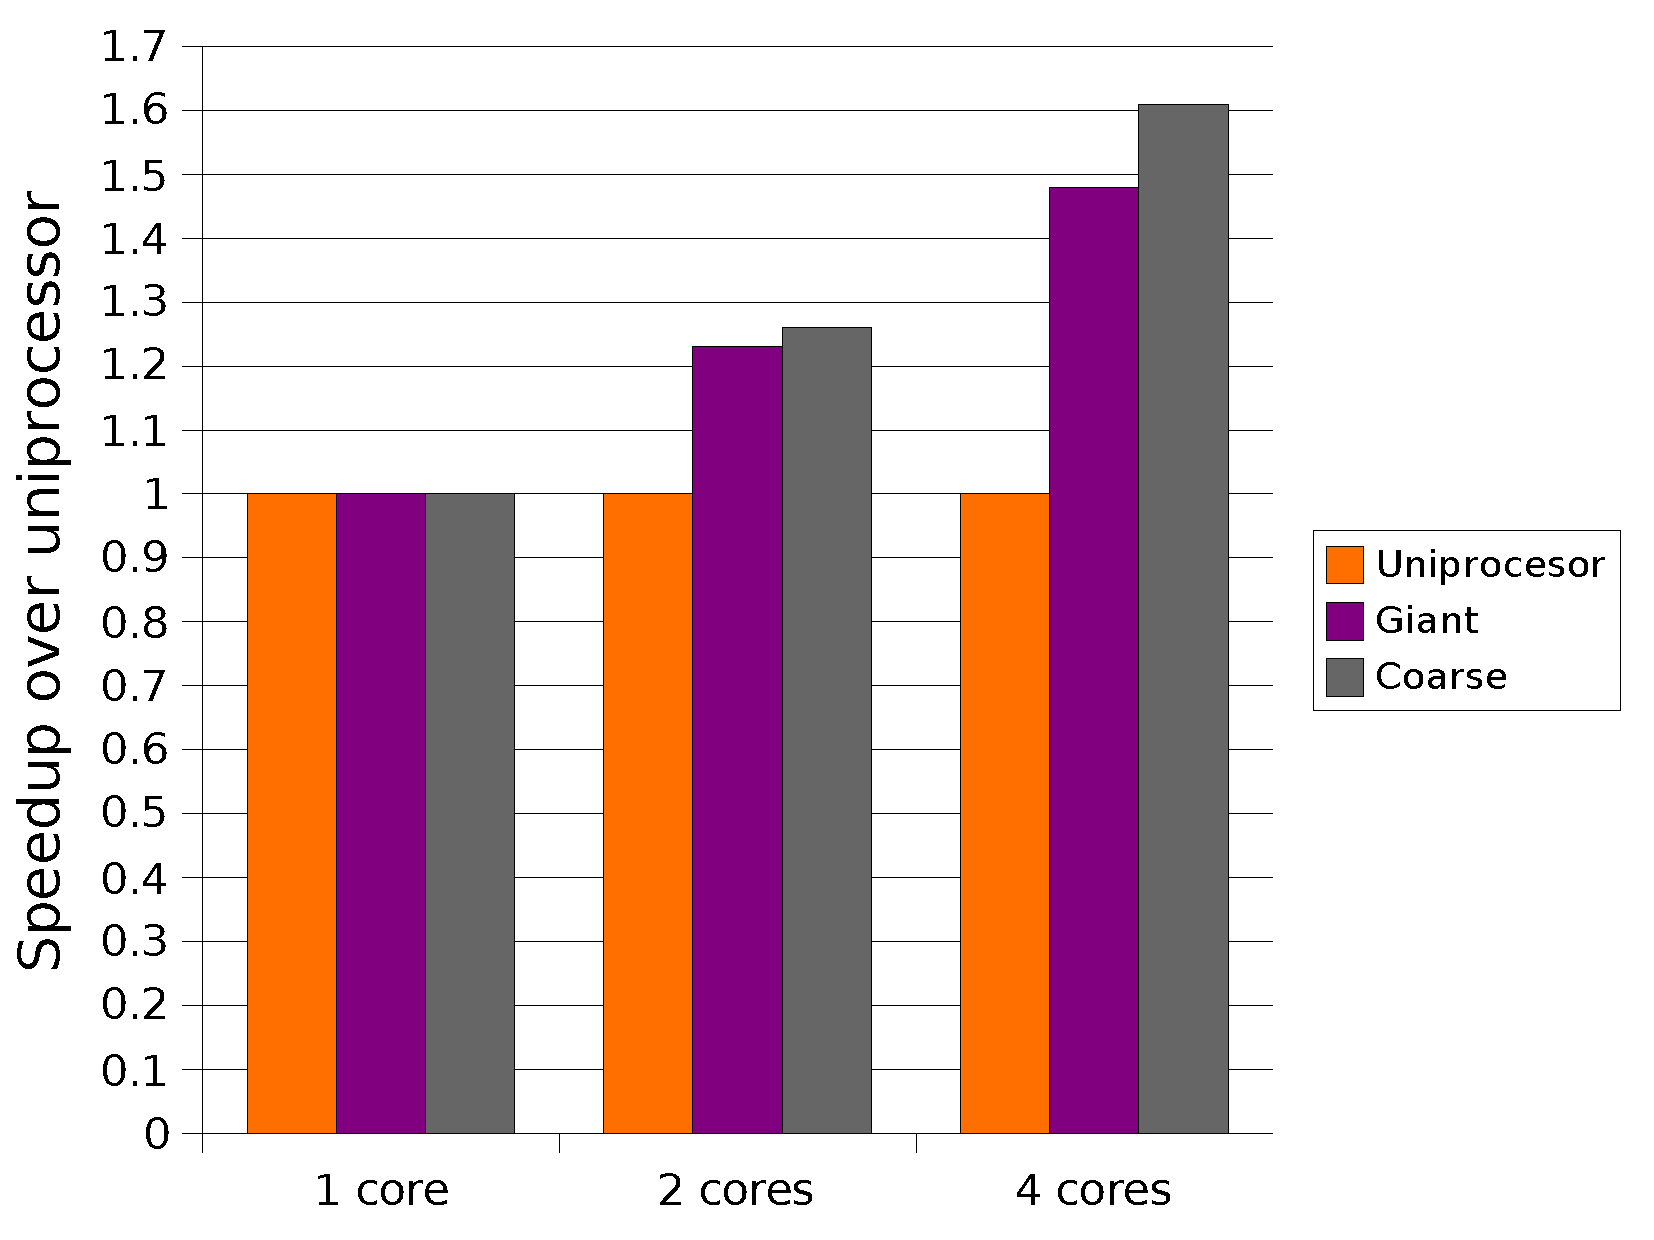
\includegraphics[width=0.8\linewidth]{figures/tsp-smp-coarse/refapp}
    \caption[C++ traffic performance results]{Performance results for the three kernel versions for C++ traffic.}
    \label{fig:dicos-cg:cpp-results}
  \end{center}
\end{figure}

\begin{figure*}[thb]
  \begin{center}
    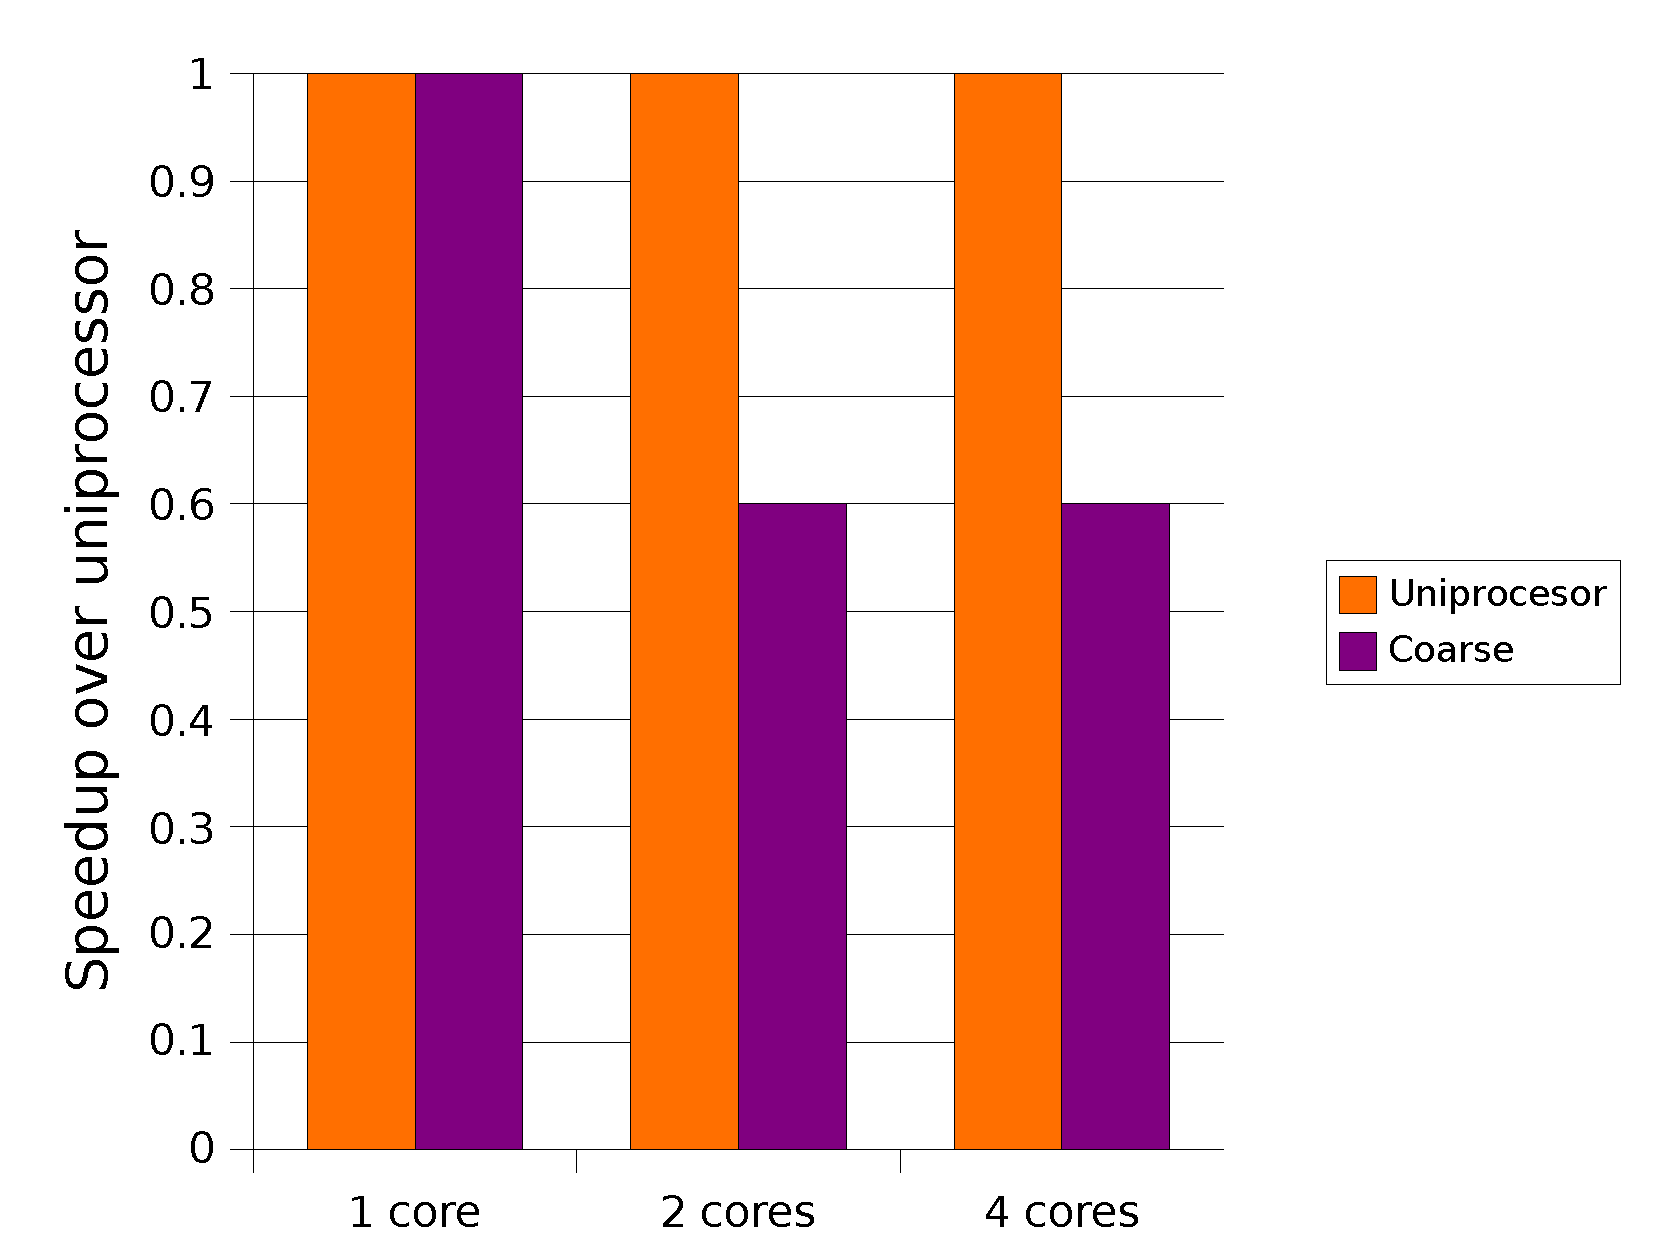
\includegraphics[width=0.6\linewidth]{figures/tsp-smp-coarse/java-no-lfh}~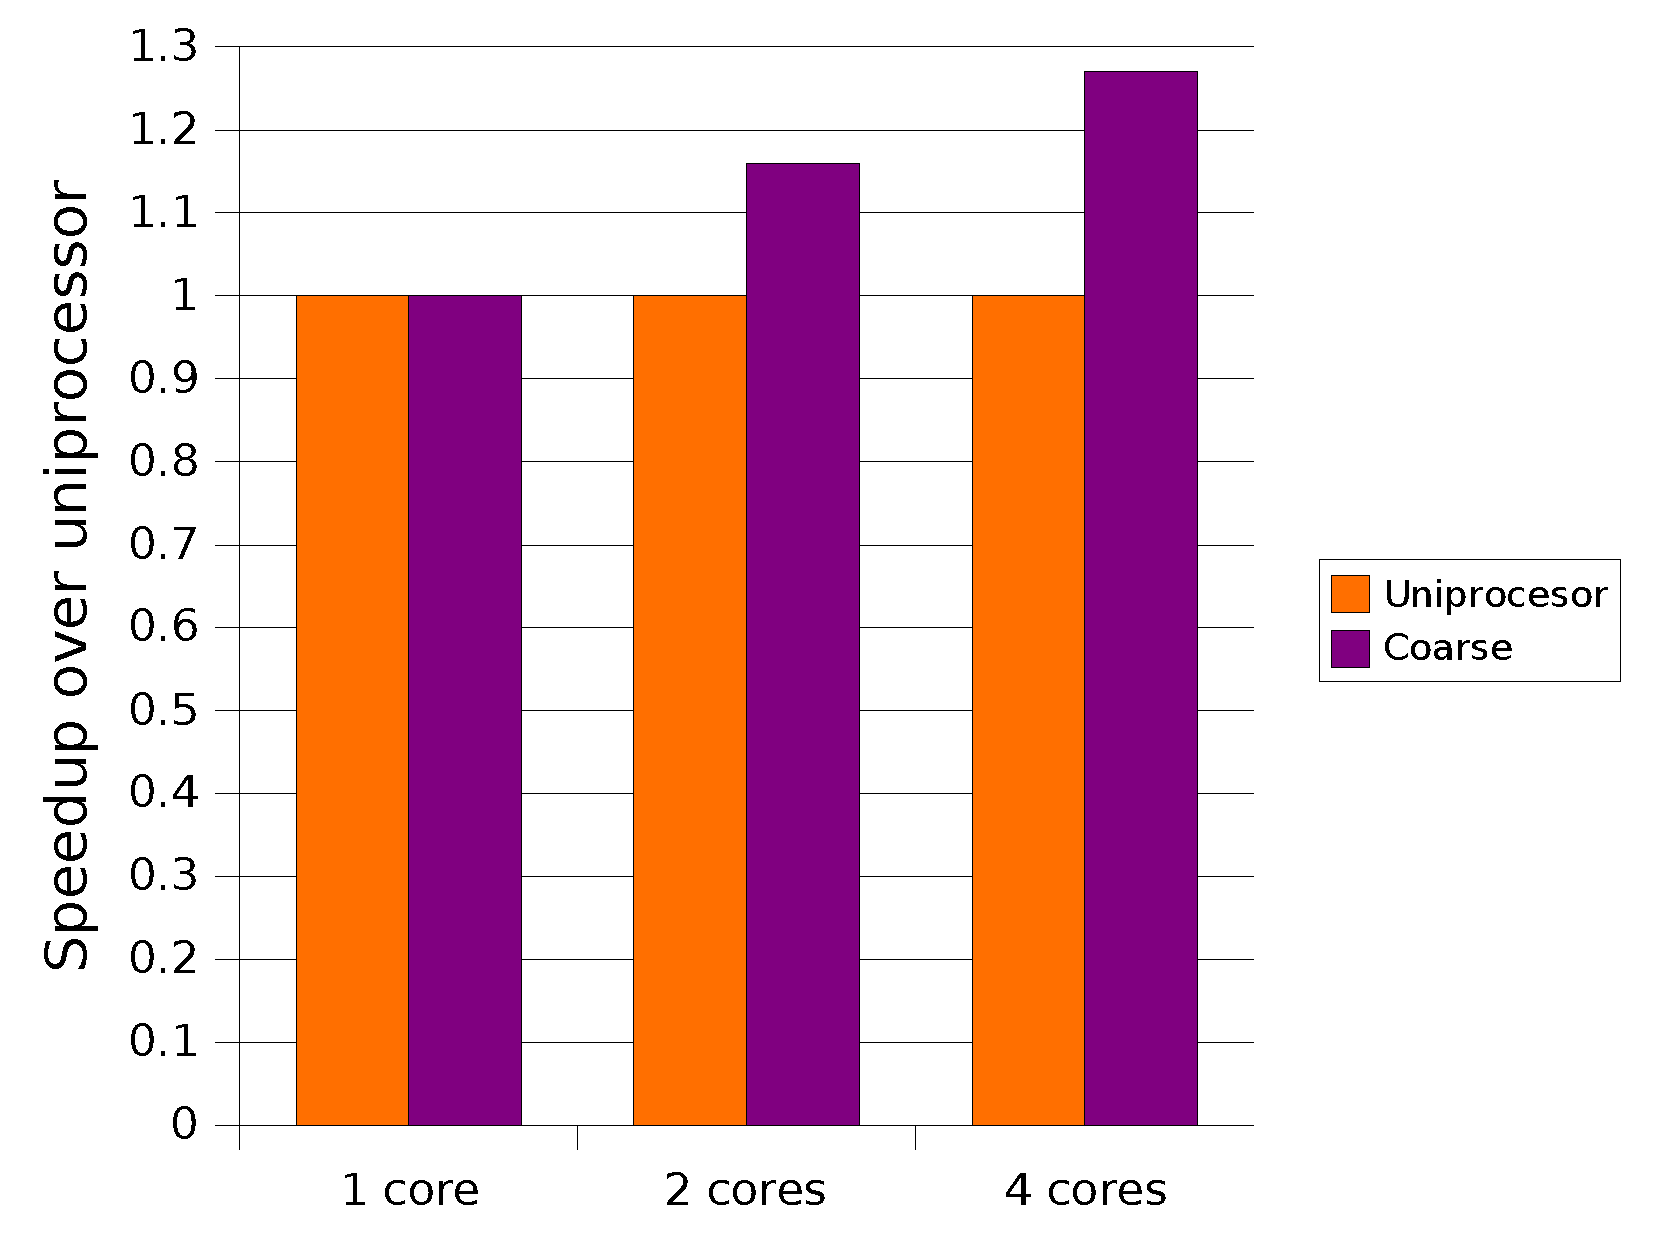
\includegraphics[width=0.6\linewidth]{figures/tsp-smp-coarse/java-lfh}
    \caption[Java traffic performance results]{Performance results for the three kernel versions for Java
      traffic. The left part of the figure shows the standard heap and the
      right shows the lock-free heap}
    \label{fig:dicos-cg:java-results}
  \end{center}
\end{figure*}

We measure at what level of calls per second the load of the system reaches
100\%, i.e., at what level the system cannot accept more work. The results are
anonymized and shows the speedup compared to uniprocessor operation. The test
runs with two kernels, one which holds the giant lock for all operations and
one which uses the coarse-grained locking implementation. The uniprocessor
version runs with all locks inactive, but contains the same memory management
implementation. The tests were performed on a 4-CPU machine with two dual-core
2.8GHz AMD Opterons.

The results for C++ traffic are shown in
Figure~\ref{fig:dicos-cg:cpp-results}. As the figure shows, the improvement
compared to the uniprocessor is around 20\% for the 2-core case with the giant
lock and 48\% for the 4-core case. For the coarse-grained locking, the
performance improvement compared to the uniprocessor is almost 23\% and 61\%
for the 2 and 4-core cases, which shows that the coarse-grained approach gives
some benefits over the pure giant lock. We expect that these numbers will
improve when the database has been separated to use it's own locks.

Figure~\ref{fig:dicos-cg:java-results} shows the results for Java traffic with
and without the lock-free heap for the uniprocessor and the coarse-grained
implementation. As the left part of the figure shows, the heap problems makes
performance deteriorate on multiprocessor configurations. Since threads are
almost always blocking on the heap semaphores, threads are effectively
serialized and multiple CPUs will only cause overhead. There is also no
scaling when going from two to four cores, which is also caused by the
serialized threads. The right part of the figure shows the results with the
lock-free heap. As can be seen in this figure, there is an improvement both in
the two- and four core cases, albeit not as much as with C++ traffic. The
results also scale between the two- and four core case. Again, we expect that
the performance will improve with the database lock.

\section{Related work}
\label{sec:dicos-cg:related}

The cluster-based operating system we are working with is perhaps most similar
to the Plurix operating system~\cite{goeckelmann03plurix}. Plurix is a
Java-based operating system which provides distributed shared memory with
communication through shared objects. The distributed in-RAM database in the
operating system serves a similar purpose, but is not implemented through
distributed shared memory. Also, the Plurix kernel only runs on uniprocessor
hardware and only supports a Java runtime environment whereas we support
multiprocessors and C++ as well and use a kernel written in C++.

There have been several ports of uniprocessor kernels targeting multiprocessor
systems. AIX~\cite{clark95symmetric, talbot95aix} was ported to multiprocessor
PowerPC hardware around 10 years ago. The port lasted around 18
months~\cite{talbot95aix} and totally involved more than 100 people, although
this includes other work for the next AIX release. Similar to our
implementation, the AIX developers used a mix between fine-grained and
coarse-grained locks, with some subsystems being locked by coarse-grained
locks and more performance critical ones using fine-grained locks. A
difference is the AIX kernel already allowed in-kernel thread preemption,
which means that the uniprocessor base already deals with some of the problems
we encountered. AIX locks can also block threads so that the CPU switches to
another thread. This is not possible in general with our kernel since it does
not allow kernel thread preemption.

Solaris~\cite{kleinman92solaris}, Linux~\cite{beck98linux},
FreeBSD~\cite{lehey03freebsd} have also been ported to multiprocessor systems.
For Linux and FreeBSD, the initial versions used a giant locking scheme
similar to our prototype. Their locking schemes have later been refined to
implement more fine-granular approaches, starting with coarse-grained locks
and gradually moving to fine-grained locking. The Solaris implementation
immediately moved to a fairly fine-grained locking approach.

The problem with heap allocators on multiprocessor platforms has been studied
in several earlier articles~\cite{haggander98icpp, haggander00pdcs,
  haggander99part, michael04pldi}. For applications which does frequent heap
allocations, introducing a multithreaded or lock-free heap can give
significant advantages. Our experience validates this observation and also
illustrates behavioral differences in multithreaded programs on uniprocessors
and multiprocessors.

There are also some alternative approaches to multiprocessor porting. For
example, the application kernel approach~\cite{kagstrom05appkern} describes a
method where a small \emph{application kernel} is installed as a loadable
module beside the regular kernel, and handles all CPUs except the boot CPU.
Applications thereafter run on the application kernel, but system calls are
forwarded to the boot CPU and handled by the original kernel. This approach
allows a multiprocessor port without changing the original kernel, but limits
scalability of kernel-bound work and is therefore unlikely to provide good
results for the operating system we are targeting. Virtualization is another
possible approach to benefit from a multiprocessor. Cellular
Disco~\cite{govil99cellular} partitions a large multiprocessor into a virtual
cluster, and runs multiple IRIX instances in parallel. However, virtualization
would require the high availability framework for the operating system to
change in order to avoid co-location of database objects on the same node. We
also investigated a port to the paravirtualized Xen system~\cite{barham03xen},
but for technical reasons it turned out to be difficult to implement.

\section{Conclusions}
\label{sec:dicos-cg:conclusions}
In this paper, we have described experiences from porting an operating system
kernel to multiprocessor hardware. We have outlined the implementation of
coarse-grained locking for the kernel, which is based on a prototype with a
giant lock that serializes kernel execution. We have also described the most
important problems which arose and our solutions to these. Our evaluation
shows that the coarse-grained approach improves on the giant locking approach
for the kernel-bound workload we target.

The prototype giant lock implementation has many similarities with the
uniprocessor implementation. Processes executing in the kernel are never
interrupted, so the original uniprocessor semantics are mostly kept
unmodified. The changes for the implementation were mostly related to CPU
startup and CPU-local data and the implementation of multithreaded address
spaces. After the initial implementation, correctness was therefore not a big
problem with the giant locking approach.

For the coarse-grained implementation, the changes to the uniprocessor base
are much larger. With multiple CPUs executing concurrently in the kernel, many
of the assumptions made in the uniprocessor implementation are no longer true.
While some of these problems were found and analyzed during the
prestudy-phase, e.g., the problems with multithreaded termination, others were
not found until we started prototyping the implementation. For example, we
first made the idle loop immediately enter the scheduler again to keep CPUs
busy, but since this was shown to cause a high contention on the giant lock we
revised the implementation. The heap locking problem, which actually occurs in
user-space, was similarly unexpected and was caused as an indirect effect of
true multithreading.

Our experiences illustrates the diversity of problems associated with
multiprocessor ports of operating system kernels. Since the changes affect
large parts of the code base, with parallelization of many parts of the
kernel, this type of port requires thorough knowledge of a large set of
modules in the kernel. In general, the difficult problems have occurred in
parts of the code that were not directly changed by the multiprocessor port.
For example, most of the timer code is not directly affected by the
multiprocessor port, yet it has caused several difficult indirect problems in
code that uses the timers.

While we've had a set of difficult problems during the implementation of the
coarse-grained locking approach, the duration of the project have still been
shorter than the giant lock prototype, which took almost two
years~\cite{kagstrom05experiences}. The primary reason is that the prototype
was implemented by a single developer without previous experience with the
operating system working part-time at a remote site, while the coarse-grained
approach was implemented by a team of experienced designers working on-site.
Another reason is simply that we could start from the already working giant
locking implementation and work incrementally from that, which has enabled the
development to continue in small steps. A third reason has been the improved
tool support, primarily the use of GDB through Qemu, which was not available
when the giant lock prototype was developed.

\section*{Acknowledgements}
This work was partly funded by The Knowledge Foundation in Sweden under a
research grant for the project ``Blekinge - Engineering Software Qualities
(BESQ)'' (\url{http://www.bth.se/~besq}).

%We would like to thank the anonymous reviewrs for their valuable input

%%% Local Variables: 
%%% mode: latex
%%% TeX-master: t
%%% End: 
